\documentclass{article}

\usepackage[utf8]{inputenc}
\usepackage[pdftex]{graphicx}
\usepackage[left=3cm,right=3cm,top=3cm,bottom=3cm]{geometry}
\usepackage[T1]{fontenc}
\usepackage[francais,english]{babel}
\frenchbsetup{StandardLists=true}
\selectlanguage{english}


\usepackage{amsmath}
\usepackage{amssymb}
\usepackage{mathtools}
\usepackage{slashbox}


\usepackage{caption}
\usepackage[hidelinks]{hyperref}
\usepackage{xcolor}


%ALGORITHM
\usepackage{algorithm}
\usepackage[noend]{algpseudocode}
\renewcommand{\algorithmicforall}{\textbf{for each}}
\newcommand{\var}[1]{\mathit{#1}}
\newcommand{\func}[1]{\mathrm{#1}}
\algdef{SE}[DOWHILE]{Do}{doWhile}{\algorithmicdo}[1]{\algorithmicwhile\ #1}
%

\usepackage{listings}

\usepackage{graphicx}

\renewcommand\thesection{\arabic{section}}

\usepackage{fancyhdr}
\pagestyle{fancy}
\fancyhf{}
\fancyhead[R]{\thepage}


\title{[INFO-F409] Learning Dynamics \\ Second assignment}
\author{\bsc{BUI QUANG PHUONG} Quang Linh \\ Université libre de Bruxelles - ULB ID : 000427796  \\ MA1 Computer Sciences}
\date{December 2018}

\begin{document}

\maketitle

\tableofcontents

\newpage
\section{Part I: Complex networks}

\subsection{1 - Erdos-Renye network}

\subsubsection{Q1 statement}

\textit{Generate Erdos-Renye network (Random networks) [1,2]. Generate the network from scratch and present/describe the part of the code you used to generate the network in your document. For a size of the network of N=10000, calculate a K so that each node has in average degree 4.} 

\subsubsection*{Pseudo-code}

\begin{algorithm}
  \caption{Generation of Erdos-Renye network}\label{euclid}
  \begin{algorithmic}[1]
  \Procedure{ErdosRenye}{$n$, $K$}
  \State Initialize the network edges list
  \ForAll{'future' edges $\equiv 0 \rightarrow K$}:
  \State Pick two random nodes in the network
  \State Define $newEdge$ variable taking the 2 picked nodes  
  \EndFor
  \If {$newEdge$ not already exists}:
  \State Add $newEdge$ in the list of edges
  \EndIf
  \Return list of network's edges  
  \EndProcedure
  \end{algorithmic}
\end{algorithm}

\subsubsection*{Algorithm description} 

The Erdos-Renye network is a random network generated. Before all, we have to initialize a list of edges which will be returned and will form the random network. This edges list is composed by some tuples of 2 elements $(x,y)$ representing the edges where $x,y$ are the two nodes that the edge is connecting. Now, we have to keep creating edges while the number edges $K$ passed in parameters isn't reached. The random part is managed by the step of picking nodes by pair $(x,y)$ in the network which is totally random, all nodes can be picked at this moment. Of course, before accepting the edge between de two nodes chosen, a verification that this edge doesn't already exists, which means that the edge $(x,y)$ \textbf{\underline{and}} $(y,x)$ isn't already created, is done.

\subsection*{K for average degree of 4}

To calculate the value of $K$ for an average degree of 4, first we know that an edge generates a link between two nodes and then increases the degree of two nodes. Moreover, we have 10000 nodes, thus we can calculate the value of $K$ for an average degree of 4 using the following formula : $ \frac{2K}{10000} = 4 $ that gives $K = 20000$. 

\subsubsection{Q2 statement}

\textit{Plot the degree distribution of the generated network. Calculate the mean and standard deviation and plot the normal distribution with these same parameters}

\subsubsection*{Degree distribution} 
The degree distribution of the network generated by the Erdos-Renye algorithm with $K = 20000$ is given by the \autoref{fig:ER-distribution}. 

\begin{figure}[h]
  \centering
  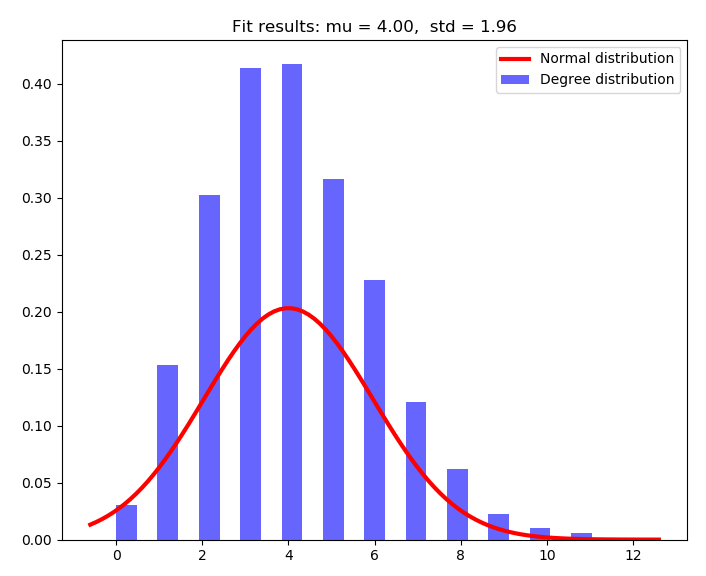
\includegraphics[scale=0.35]{fig/ER-distribution.png}
  \caption{Distribution for Erdos-Renye generated network}
  \label{fig:ER-distribution}
\end{figure}

\subsubsection*{Mean and standard deviation}
The value of the mean in the distribution of \autoref{fig:ER-distribution} is 
$$ \mu = 3.998 $$ and for the standard deviation is $$ \sigma = 2.012 $$. 

\subsection{2 - Barabasi-Albert network}

\subsubsection{Q3 statement}
\textit{Generate a Barabasi-Albert network (Scale Free network) [1,3]. Generate the network from scratch and present/describe the part of the code you used to generate the network in your document.}

\subsubsection*{Pseudo-code} 

\begin{algorithm}
  \caption{Generation of Barabasi-Albert network}\label{euclid}
  \begin{algorithmic}[1]
  \Procedure{BarabasiAlbert}{$Graph$, $N$}
  \State Initialize a fully connected 4 nodes network
  \ForAll{'future' node until $N \equiv 4 \rightarrow N$}:
  \State Add a node $x$ to the network 
  \ForAll{current network's nodes}:
  \State Compute the probability of the added node $x$ being linked to those nodes
  \State Append it into a list $probasLinking$  
  \EndFor
  \State Pick 4 nodes with their associated probabilities just computed before in the network's nodes
  \For{the 4 picked nodes}:
  \State Link the added node $x$ to them
  \EndFor
  \EndFor
  \State Reinitialize $probasLinking$ and increment by 8 (4 new edges = 8 nodes with their degree increasing by 1) the total degree number for the computation of the next probabilities 
  \EndProcedure
  \end{algorithmic}
\end{algorithm}

\subsubsection{Q4 statement}
\textit{Plot the degree distribution of the generated network using a linear scale on both axes. Plot in the same figure an exponential distribution which looks similar and reports on the parameters of that distribution.}

\subsubsection*{Degree distribution result (linear scale)} 

\subsubsection*{Exponential distribution} 

\subsubsection{Q5 statement}
\textit{Plot the same distribution on log-log scale. Fit the distribution using Least Square fit. You can use existing functions for fitting and plot the fit next to the data. What are the parameters of the fit? How does it fit? Why? Write a paragraph about why we should not use Least Square fit to fit power laws.}

\subsubsection*{Distribution on log-log scale} 

\subsubsection*{Fitting using Least Square Fit} 

\subsubsection{Q6 statement}
\textit{Plot cumulative distribution and fit it with Least Square Fit, report the obtained parameters and plot of the fitted function.}

\subsubsection*{Plotting result and parameters} 

\subsubsection{Q7 statement}
\textit{Now fit your distribution using maximum likelihood method. You can use any of the packages which has the method developed.}

\subsubsection{Q8 statement}
\textit{Report the parameters of the fit and plot them next to distribution.}

\subsubsection{Q9 statement}
\textit{Compare the power law fit with the exponential fit (using the same package). Report the log likelihood ratio R and the p-value. What do these numbers mean?}

\subsubsection{Q10 statement}
\textit{What is the mathematical formula for scale free distribution you generated? Calculate the mean and the standard deviation of function? What would be the mean and standard deviation if the exponent would be 2.5?}


\end{document}